\xchapter{Problemas de escalonamento e roteamento}{ }
%Este capítulo apresenta a formulação do problema, as principais definições para o entendimento do mesmo e um resumo de todo o material estudado.}

\presetkeys%
    {todonotes}%
    {inline,backgroundcolor=yellow}{}
% \todo{}


\section{Problema de Alocação de Pessoal}

O Problema de Alocação de Pessoal consiste em atribuir um conjunto de tarefas a um conjunto de pessoas, satisfazendo a um conjunto de restrições \cite{blochiger:2003}.

%O escalonamento de pessoal deve ser realizado de forma que o serviço esteja disponível durante todo o tempo previsto pela organização. Caso o trabalho de uma equipe não interfira ou não dependa do trabalho de outra equipe, então as equipes podem ser escalonadas de forma independente, caso exista alguma relação de dependência, as equipes devem ser escalonadas levando em consideração estas relações \cite{blochiger:2003}.

Seja um conjunto de pessoas $S = \{s_1,s_ 2, ..., s_{|S|}\}$ e um conjunto de tarefas  $F = \{f_1, f_2, ..., f_{|F|}\}$. Uma solução para o Problema de Alocação de Pessoal, também conhecido como \textit{Staff Scheduling}, pode ser representado por uma matriz $M$, na qual cada linha representa uma tarefa que deverá ser executada por uma pessoa $s \in S$ e cada célula $m_{f,s}$, contém o valor referente a atribuição da tarefa $f \in F$ à pessoa $s \in S$.

A Tabela \ref{time_table_block}, representa um exemplo da alocação de um conjunto de tarefas a um conjunto de pessoas de forma que cada tarefa é associada a uma pessoa, sendo que o valor $1$ na célula $m_{fs}$ indica que a pessoa $s$ deve executar a tarefa $f$, caso contrário o valor na célula $m_{fs}$ será 0.

\begin{table}[h]
\centering
\caption{Exemplo de alocação de um conjunto de tarefas a um conjunto de pessoas. \label{time_table_block}} 
\begin{tabular}{r|l|l|l|l}
   & $s_1$ & $s_1$ & $s_3$ & $s_4$ \\ \hline
$f_1$ & 0  & 0  & 1  & 0  \\ \hline
$f_2$ & 1  & 0  & 0  & 0  \\ \hline
$f_3$ & 0  & 0  & 0  & 1  \\ \hline
$f_4$ & 0  & 1  & 0  & 0 
\end{tabular}
\end{table}

% O Problema de Alocação de Pessoal pode ser solucionado a partir da variável de decisão $X_{sf}$ , de forma que se o valor alocado for 1, significa que o item foi alocado na tabela e se for 0, significa que o item não foi alocado. 

% Na equação \ref{alocacao_pessoal}, é representada uma solução para uma instância do problema de alocação de pessoal sendo que $X$ denota o conjunto de todas as variáveis de decisão.

%   \begin{equation}
%   \label{alocacao_pessoal}
%   X_{sf} = 
%   \left \{
%   \begin{array}{cc}
%   1, & \mbox{se a pessoa $s$ foi alocada a atividade $f$} \\
%   0, & \mbox{caso contrario} \\
%   \end{array}
%   \right.
%   \end{equation}

\subsection{Problema de Alocação de Equipe Técnica}
%UMA ABORDAGEM OTIMIZADA PARA O PROBLEMA DE ALOCAÇÃO DE EQUIPES E ESCALONAMENTO DE TAREFAS PARA A OBTENÇÃO DE CRONOGRAMAS EFICIENTES
Seja $k \in K=\{k_1, k_2, ..., k_{|K|}\}$ um conjunto de equipes e $F = \{f_1, f_2, ..., f_{|F|}\}$ um conjunto de tarefas. O Problema de Alocação de Equipe Técnica \ac{PAET}, também conhecido como \ac{CSP} consiste em alocar um conjunto de equipes $K$ a um conjunto de tarefas $F$ \cite{Beasley:1996}. 

Esse problema leva em consideração que todas as equipes são idênticas e estão localizadas no mesmo depósito a partir do qual eles começam e terminam seu dia de trabalho, o número de equipes não pode ser maior do que o número de tarefas que serão executadas e o tempo de execução do conjunto de tarefas não pode exceder o tempo total $T$ \cite{Beasley:1996}.

Para cada tarefa $f$ é associada um custo de execução, uma janela de tempo $[e_f, l_f]$, sendo $e_f$ o tempo de início da execução de cada tarefa $f$ e $l_f$ o tempo final, implicando na duração de tempo $l_f - e_f$, um tempo de viagem $/tau$ e custo $c$ envolvido na viagem da da equipe do depósito para a tarefa $f$ e vice-versa \cite{Beasley:1996}.

Sem perda de generalidade, devemos assumir que as tarefas foram numeradas na ordem ascendente do início. Cada duas tarefas $i$ e $j$, com $j > i$ existe um arco de transição de custo $c_{ij}$, se for possível para a mesma equipe executar a tarefa $i$ e depois executar a tarefa $j$. As tarefas são organizadas de forma a criar um caminho de tarefas que serão executadas pela mesma equipe \cite{Beasley:1996}. 

O objetivo do problema é, encontrar caminhos de custo total mínimo, de modo que cada tarefa seja realizada exatamente uma vez e o tempo de trabalho total envolvido em cada caminho onde, por tempo de trabalho, (significamos o tempo decorrido entre a saída do depósito e a chegada de volta ao depósito) não excede o tempo de trabalho disponível T \cite{Beasley:1996}.

%Uma modelagem para o \ac{CSP} pode ser representada a partir de um grafo $G = (V, A)$, sendo cada tarefa representadas por um vértice, que estão todos ligados entre si por arestas de transição. Existindo dois depósitos mostrados como $0$ para representar o início do caminho e como $N+1$ para representar o fim do caminho. Devido a dimensão do tempo, não existem ciclos no grafo \cite{Beasley:1996}. 
%checar referência
% O objetivo do problema é encontrar os caminhos disjuntos de $K$ vértices no caminho entre $0$ e $N+1$, de modo que todas as tarefas estejam em um caminho, o tempo de trabalho incluído em cada caminho não exceda o tempo total $\tau$, o custo total dos caminhos seja mínimo.
%checar referência
%como pode ser visto na figura \ref{CSP}.

% \begin{figure}[h]
% \centering
% \caption{Exemplo Crew Scheduling Problem com K = 1}
% \centering
% 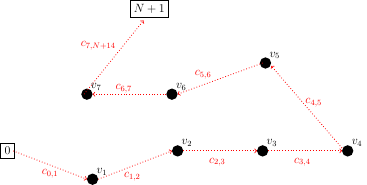
\includegraphics[width=0.8\textwidth]{CSP.png}
% \label{CSP}
% \begin{center}
% Fonte: Elaborada pelo autor
% \end{center}
% \end{figure}

%O objetivo do \ac{CSP} é encontrar todos vértices entre $0$ e $N+1$, tais que todas as tarefas estejam no mesmo caminho, o tempo de trabalho não exceda o tempo total $T$ e o custo total do caminho determinado pelas tarefas executadas seja mínimo. 
% Levando em consideração que cada tarefa pode ser executada apenas uma vez, o custo total associado a cada solução viável é definido pela soma dos custos para realizar cada tarefa $f$, como pode ser visto equação \ref{eqsum}:

% \begin{equation} \label{eqsum}
% 	\sum_{i=1}^{F} c_{f}
%  \end{equation}

% Uma aplicação prática do Crew scheduling problem é o  \textit{Home Care Crew Scheduling Problem}, é um problema no qual uma equipe do \ac{HHCSP} realiza uma série de visitas às casas dos pacientes \cite{rasmussenm:2012}.
%e deve ser encontrado uma solução ótima de forma que todas as visitas sejam feitas no menor tempo possível sem prejudicar a qualidade do atendimento. Este problema foi classificado pelo autor como NP-completo, pois foi verificado a viabilidade em reduzi-lo ao problema do caixeiro viajante, dessa forma, para resolver o problema o autor desenvolveu um algoritmo \textit{branch-and-price}. 

% Uma instância qualquer do problema geral de alocação de equipes pode ser solucionada a partir da variável de decisão $X_{fk}$, tais que, o valor $1$ é associado a uma ligação entre dois vértices, e o valor $0$ determina que não existe uma ligação entre os vértices. Como podemos ver na equação \ref{eqcsp}, que recebe o valor $1$ caso a tarefa $f$ seja associada a equipe $k$ e o valor $0$ caso contrário.

%   \begin{equation} \label{eqcsp}
%   X_{fk} = 
%   \left \{
%   \begin{array}{cc}
%   1, & \mbox{se existe a tarefa $f$ foi alocada a equipe $k$}  \\
%   0, & \mbox{caso contrario} \\
%   \end{array}
%   \right.
%   \end{equation}
  
% A tabela \ref{tarefa_equipe} ilustra um exemplo da solução para o problema de alocação de equipes, no qual cada tarefa $k$ é associada a uma equipe $e_{i}$. 

% \begin{table}[h]
% \centering
% \caption{Tabela: Tarefa X equipes}
% \label{tarefa_equipe}
% \begin{tabular}{l|l|l|l|l}
%    & k1 & k2 & k3 & k4 \\ \hline
% e1 & 0  & 1  & 0  & 0  \\ \hline
% e2 & 0  & 0  & 0  & 1  \\ \hline
% e3 & 0  & 0  & 1  & 0  \\ \hline
% e4 & 1  & 0  & 0  & 0 
% \end{tabular}
% \end{table}

% \subsection{Problema de Alocação de Recursos}

% O problema geral de alocação de recursos consiste em conjunto $R = \{1, 2, ..., r\}$ de recursos que serão escalonados; um custo $c_{r}$ representando o tempo que cada recurso permanecerá alocado, e  um conjunto de processadores  $\Omega = \{1,2, ..., \omega \}$ \cite{ullman:1975}. 
% Como podemos ver na tabela \ref{alocacao_recurso}, no qual o valor é $1$ quando o recurso é alocado no processador $p$ e $0$ quando não é alocado no processador $p$. O objetivo deste problema é executar $k$ recursos dentro do tempo $t$.

% \begin{table}[h]
% \centering
% \caption{Tabela Recurso X Processador \label{alocacao_recurso}}
% \begin{tabular}{l|l|l|l|l}
%    & $\omega1$ & $\omega2$ & $\omega3$ & $\omega4$ \\ \hline
% r1 & 0  & 1  & 0  & 0  \\ \hline
% r2 & 0  & 0  & 0  & 1  \\ \hline
% r3 & 0  & 0  & 1  & 0  \\ \hline
% r4 & 1  & 0  & 0  & 0 
% \end{tabular}
% \end{table}

% O problema de alocação de recursos pode ser solucionado a partir de uma variável de de decisão $X_{r\omega}$, sendo o valor $1$ é atribuído caso o recurso seja associado ao processador, e $0$ se não foi atribuído, como podemos ver na equação \ref{alocacao_recurso}.

%   \begin{equation}
%   \label{alocacao_recurso}
%   X_{rp} = 
%   \left \{
%   \begin{array}{cc}
%   1, & \mbox{ se o recurso $r$ foi alocado ao processador $p$}  \\
%   0, & \mbox{caso contrario} \\
%   \end{array}
%   \right.
%   \end{equation}

\section{Problema do caixeiro viajante}

O Problema do Caixeiro Viajante, também conhecido como \ac{TSP}, é um problema de otimização combinatória no qual, dado um conjunto de cidades e as distâncias estre elas, o objetivo é encontrar o caminho mais curto possível que visite cada cidade exatamente uma vez \cite{goyal:2010}.

Seja um grafo $G = (V,A)$ no qual $V$ é um conjunto de vértices e A é um conjunto de arestas, e seja $C = (c_{ij})$ uma matriz de distância (ou custo), associada com $A$. O \ac{TSP} consiste em determinar um circuito de distância mínima que passa por cada vértice apenas uma vez. Esse circuito é conhecido como um circuito Hamiltoniano \cite{laporte:1992}.

São estudadas diversas variações do \ac{PCV} existindo várias aplicações práticas para o problema, porém neste trabalho serão descritos o Problema Múltiplo do Caixeiro Viajante e do Problema o Caixeiro Viajante com Janela de Tempo. 

O \ac{PMCV}, tem como objetivo determinar um conjunto de rotas de custo mínimo que serão percorridas por um conjunto de Caixeiros Viajantes.

Uma solução para o \ac{PMCV} pode ser representada a partir de um grafo $G = (V,A,W)$ um grafo conectado, onde $V = \{v_1, v_2, ..., v_{|V|}\}$ é um conjunto de cidades, e $A = \{ v_i,v_j: v_i,v_j \in V, i \neq j\}$ é uma aresta com uma matriz custo não negativo $C = {c_{ij}: o peso de (v_i,v_j)}$. $c(v_i, v_j)$ é a distância entre $v_i$ e $v_j$, denotada por $w_{ij}$. d(i) denota o número de arestas conectadas a um vértice $v_i$ no grafo. Um caminho é denotado por uma rota entre dois nós finais com grau 1. Um circuito indica uma rota que começa e termina no mesmo nó. 
\cite{meng:2012}. 

O \ac{PCVJT}, conhecido como \ac{TSPTW}, consiste em encontrar a viagem de menor custo, começando e terminando na mesma cidade e visitando todos os clientes uma única vez. Cada cliente possui um tempo de serviço definido por uma janela de tempo $[e_{i}, l_{i}]$, sendo $e_{i}$ o tempo de início e $l_{i}$ o tempo de término do atendimento. As visitas devem ser realizadas respeitando a janela de tempo.~\cite{urrutia:2010}.  

Seja $G=(V,A)$ um grafo, onde $V = \{v_0, v_1, ..., n \}$ é um conjunto de n nós, sendo $0$ o depósito e a aresta $A = {(i,j): i,j \in V, i \neq j}$. A janela de tempo é representada por $[e_i, l_i]$ e para cada aresta $(i,j) \in A$ é associado um custo $c_{ij}$ e um tempo de viagem $t_{ij}$ \cite{calvo:2000}.

O Problema do Caixeiro Viajante com o Janela de Tempo é descrito por um conjunto de clientes totalmente interconectados, cada um caracterizado por um intervalo de tempo. Um dos nós representa um depósito, e cada arco possui um tempo e custo de viagem associados. O problema consiste em encontrar um passeio Hamiltoniano de custo mínimo que visita cada nó durante sua janela de tempo. O passeio começa e termina no depósito \cite{calvo:2000}.

\section{Problema de roteamento de veículos}

O problema clássico de roteamento de veículos, conhecido como \ac{VRP}, tem como objetivo encontrar um conjunto de rotas com custo mínimo, começando e terminando a rota no depósito, de modo que seja cumprida a demanda dos clientes. Cada local é visitado uma vez, e cada veículo possui uma capacidade limitada \cite{gold:2008}.

Seja um conjunto de clientes $Q = \{q_1, q_2, ..., q_{|Q|}\}$, que residem em locais $W = \{w_0, w_1, w_2, ..., w_{|W|}\}$ diferentes. Cada par de locais $(i,j)$, onde  $i,j \in W$ e $i \neq j$, é associado a um tempo de translado $\tau$ e uma distância $u_{ij}$. O depósito, local de onde os veículos partem e retornam, é denotado por $w_0$.
Os clientes são atendidos a partir de um depósito com uma frota  homogênea $Z = \{1, 2, ..., z_{|Z|}\}$ de veículos com capacidade uniforme $y$~\cite{gold:2008}.

O Problema de Roteamento de Veículo com Janela de tempo, o \ac{VRPTW}, assim como o \ac{VRP}, consiste em encontrar um conjunto de rotas com custo mínimo, porém cada cliente $q$ possui uma janela de tempo $[e_{q}, l_{q}]$, sendo $e_{q}$ o tempo de início do atendimento e $l_{q}$ o tempo do fim do atendimento~\cite{gold:2008}.